%\documentclass[10pt,twocolumn,twoside]{IEEEtran}
\documentclass[journal]{IEEEtran}

% The following packages can be found on http:\\www.ctan.org
\usepackage{graphics} % for pdf, bitmapped graphics files
\usepackage{epsfig} % for postscript graphics files
\usepackage{mathptmx} % assumes new font selection scheme installed
\usepackage{times} % assumes new font selection scheme installed
\usepackage{amsmath} % assumes amsmath package installed
\usepackage{amssymb}  % assumes amsmath package installed
\usepackage{algorithm}
% \usepackage[utf8]{inputenc}
\usepackage[noend]{algpseudocode}
\usepackage{graphicx}
\usepackage[font=small,labelfont=bf]{caption}
\usepackage{epsfig}
\usepackage{ulem}
\usepackage{verbatim}
\usepackage{amsfonts}
\usepackage{mathrsfs}
\usepackage{breqn}
\usepackage{xcolor}
\usepackage{mathtools}
\DeclarePairedDelimiter{\ceil}{\lceil}{\rceil}
\newcommand{\qd}{\hfill{\qed}}
\def\ba{\begin{array}}
\def\ea{\end{array}}
\newcommand{\beq}{\begin{equation}}
\newcommand{\eeq}{\end{equation}}
\newcommand{\bq}{\begin{eqnarray}}
\newcommand{\eq}{\end{eqnarray}}
\newcommand{\bqn}{\begin{eqnarray*}}
\newcommand{\eqn}{\end{eqnarray*}}
\newcommand{\bee}{\begin{enumerate}}
\newcommand{\eee}{\end{enumerate}}


\RequirePackage{ifthen}
\usepackage{amssymb,mathrsfs,wasysym}
\usepackage{tikz}
\usepackage{url}
\usetikzlibrary{shadows}
\usetikzlibrary{shapes}

\newcommand{\always}{\square}
\newcommand{\eventually}{\Diamond}
\renewcommand{\next}{\ocircle}
\newcommand{\until}{\hspace{1mm}\mathcal{U}\hspace{1mm}}
\newcommand{\untilc}{\mathcal{U}}
\newcommand{\release}{\hspace{1mm}\mathcal{R}\hspace{1mm}}
\newcommand{\true}{\relax\ifmmode \mathit{True} \else \em True \/\fi}
\newcommand{\false}{\relax\ifmmode \mathit{False} \else \em False \/\fi}
\newcommand{\aand}{\hspace{1mm}\wedge\hspace{1mm}}
\newcommand{\oor}{\hspace{1mm}\vee\hspace{1mm}}
\newcommand{\set}[1]{\left\{#1\right\}}
\newcommand{\norm}[1]{\left\lVert#1\right\rVert}

% correct bad hyphenation here
% \hyphenation{op-tical net-works semi-conduc-tor}

\setlength{\textfloatsep}{10pt plus 1.0pt minus 2.0pt}
\begin{document}

\title{Fire Fightin' UAVs! (Not actual title...)}



\author{Joshua~Shaffer~
		and~Estefany~Carrillo% <-this % stops a space
\thanks{J. Shaffer is with the Department of Aerospace Engineering,
	University of Maryland, College Park,
	MD 20740, USA e-mail: jshaffe9@terpmail.umd.edu.}% <-this % stops a space
\thanks{E. Carrillo is with the Department of Electrical and Computer Engineering, University of Maryland, College Park,
  MD 20740, USA e-mail: ecarril2@terpmail.umd.edu.}}% <-this % stops a space


% As a general rule, do not put math, special symbols or citations
% in the abstract or keywords.

\maketitle

% As a general rule, do not put math, special symbols or citations
% in the abstract or keywords.
\begin{abstract}
Abstract will focus on the motivations of this paper, implementation and results with a brief conclusion.
\end{abstract}

% Note that keywords are not normally used for peerreview papers.
\begin{IEEEkeywords}
Controller synthesis, Allocation processes, Receding Horizon control, Linear Temporal Logic.
\end{IEEEkeywords}


% For peer review papers, you can put extra information on the cover
% page as needed:
% \ifCLASSOPTIONpeerreview
% \begin{center} \bfseries EDICS Category: 3-BBND \end{center}
% \fi
%
% For peerreview papers, this IEEEtran command inserts a page break and
% creates the second title. It will be ignored for other modes.
\IEEEpeerreviewmaketitle

\section{Introduction}
% The very first letter is a 2 line initial drop letter followed
% by the rest of the first word in caps.
% 
% form to use if the first word consists of a single letter:
% \IEEEPARstart{A}{demo} file is ....
% 
% form to use if you need the single drop letter followed by
% normal text (unknown if ever used by the IEEE):
% \IEEEPARstart{A}{}demo file is ....
% 
% Some journals put the first two words in caps:
% \IEEEPARstart{T}{his demo} file is ....
% 
% Here we have the typical use of a "T" for an initial drop letter
% and "HIS" in caps to complete the first word.

%#######################
% be more general: all electric power systems not just aircraft done
%######################
\IEEEPARstart{R}{eactive} synthesis provides a means for generating correct-by-construction controllers for complex systems. Synthesized controllers take into account varying types of dynamics for system and environment variables, progress and safety specifications, and initial conditions. The primary benefit of this method is the correct-by-construction attribute; the realized controller will always follow the specifications designed by the user as long as the environment falls within the assumptions made. Programmers are not required to “handcraft” individual behaviors of a system under specific conditions (of which are often error prone) and can instead focus on defining the system and specifications. The major pitfall of reactive synthesis, though, is the possibility of state explosion for highly granular state and environment definitions (even when the states are written in the standard GR(1) form).

Despite the aforementioned benefits, reactive synthesis is currently limited to a high-level view of systems with low granular abstractions and restrictive system and environment assumptions. Without this type of framework, most problems become infeasible to handle only with reactive synthesis. If, for example, an “open” environment (such as arbitrary obstacle placement) and a large state space (such as a 10x10 grid) were utilized to create a scenario involving the path planning of a robot that must always avoid any obstacle, synthesis of a solution would require an impractical amount of time. This stems from the fact that the synthesized controller must account for every possible environmental move ($2^{100}$ permutations for arbitrary obstacles in a 10x10 grid). Unfortunately, real problems can typically involve this scale of permutations in the environment, hence the restrictions enforced on reactive synthesis. 

When the high-level design of a system does involve this scale of environmental permutations and state space, solutions typically seek to discretize the synthesis problem or approach the problem from a different perspective. Discretization appears in the use of receding horizon control in \textcolor{red}{[CITE]} and the use of decentralized controllers for multiple agents in \textcolor{red}{[Need-based Coordination for Decentralized High-level Robot Control]}. Both examples break down the top-level synthesis problem into smaller, discrete pieces for the computation benefits. On the other hand, \textcolor{red}{[DeCastros]} approached their synthesis problem with a focus on resolving deadlock under specific environment conditions instead of directly avoiding dynamic obstacles, effectively limiting the number of permutations the reactive synthesis problem experienced and allowing lower level controllers to handle the real-time presence of dynamic obstacles. In each of the presented cases, the problem description focuses on a limited task space and how the solution can handle larger sets of actions from an environment. Specifically, in \textcolor{red}{[CITE]}, the task space encompasses \textcolor{red}{n} progress statements, in \textcolor{red}{[Need-based]}, the task space for a single robot encompasses \textcolor{red}{n} progress statements, and in \textcolor{red}{[DeCastros]}, the task space for the 2nd example encompasses 4 progress statements. 
%Even with the problem space discretized, both examples presented rely on other methods to achieve the desired results. In [CITE],... and in [CITE]... Clearly a gap still exists between designing the high-level controllers for robust autonomous systems that reside within reality and utilizing reactive synthesis to fully realize such designs. In truth, attempting to close the gap presents a futile challenge, one that .... 

This paper is motivated by the concept of combining reactive synthesis with other methods to work in tandem and provide a solution to a high-level problem with a large number of tasks to achieve. We seek to build upon the work described above by exploring a multi-agent system in a complex dynamic environment while meeting a task-space on an order of magnitude greater than the aforementioned task spaces. 

Furthermore, we aim to explore a scenario involving unmanned aerial vehicles (UAVs) and their potential benefits to fighting wildfires. Current methods of fighting fires involve numerous man hours and piloted vehicles capable of dropping large amounts of suppressant over regions of fire. As the June 2015 issue of Aerospace America discussed in the article “Firedrones” \textcolor{red}{[cite]}, UAVs of varying sizes currently pose a huge benefit to traditional firefighting methods through additional “eyes in the sky” and supply drops, and numerous agencies have spent the last decade exploring such options. While not a readily viable option, UAVs could potentially help extinguish fires on their own, as was mechanically demonstrated in \textcolor{red}{[Design and implementation]}. The scenario presented in \textcolor{red}{[Design and implementation]} dealt solely with one UAV gathering water, moving to another location, and dumping said water on the destination. These independent actions were performed through low-level controllers that were initiated by a high-level mission planner. Said mission planner, though, was not constructed to interpret the behaviors of multiple UAVs and fulfill complex specifications through its own volition, and as such, it was limited to only coordinating and enacting the lower-level controllers between two way-points. As often assumed in other sources dealing with high-level synthesized controllers, the availability of low-level controllers to dictate the motion of individual agents in real-time must exist to achieve the higher-level controller, of which are demonstrated though \textcolor{red}{[Design]}.


The rest of the paper follows as such. In \textit{Preliminaries}, we discuss subjects pertinent to the exploration of our topic. In \textit{Problem Scenario}, we present the firefighting scenario, including environment and system definitions. Additionally, we discuss the exploration of possible solutions to such a problem. \textit{Problem Solution} is dedicated to presenting our proposed solution, followed by \textit{Implementation} which details how our solution is enacted, along with the construction of our simulation for testing such. \textit{Results} present the outcomes to our tested cases, followed by the \textit{Conclusions} section.%such that reactive synthesis alone could not realize and synthesize a controller for within a limited time-frame. In the scenario, we account for the dynamics of the system within the synthesis problem. From such, a novel solution is explored which combines an allocation process with the finite automata generated from reactive synthesis operating within a receding horizon framework. The assembly of these two methods work to fully achieve the desired behavior for the constructed scenario.

\section{Preliminaries}
In this section, we provide details about the commonly used terminology, notation, and equations surrounding reactive synthesis, particularly with respect to the application in this paper. 

\subsection{Linear Temporal Logic}
To begin, linear temporal logic (LTL) is utilized for describing specifications within the reactive synthesis framework. LTL consists of infinite logic sequences upon a finite set of variables, of which make up the environment and system for this paper. Through these sequences, the behavior of a system can be described with respect to the actions of an environment.

LTL itself is built through atomic propositions, logic connections and temporal modal operators. Logic connections include $\lnot$ (negation), $\lor$ (or), $\land$ (and),  and $\longrightarrow$ (\textcolor{red}{Not sure, results?}). Temporal modal operators include $\next$ (next), $\always$ (always), $\eventually$ (eventually), and $\until$ (until). An atomic proposition (AP), $p$, is an LTL formula formed through the finite variable set, and propositional formulas (denoted with $\varphi$) consist of only logic connections on APs. Propositional formulas are also LTL formulas. %(CITE), (CITE), and (CITE) each provide more in-depth overviews of LTL, while (CITE) provides a fully comprehensive look on the subject for readers unfamiliar with LTL.
%######################

\subsection{Reactive Synthesis}
Reactive synthesis provides a method for generating controllers within the context of a defined environment and system. Specifications written in LTL are utilized to describe the desired behavior of the system and environment. One of the most commonly used forms for these LTL formulas is general reactivity(1) (GR(1)), the assume-guarantee form:
\begin{equation}
\begin{aligned}
(\varphi_{init}^{e} \land \bigwedge_{i \in I_r} \always \varphi_{s,i}^{e} \land \bigwedge_{i \in I_f} \always \eventually \varphi_{p,i}^{e}) \longrightarrow \\ (\varphi_{init}^{s} \land \bigwedge_{i \in I_s} \always \varphi_{s,i}^{s} \land \bigwedge_{i \in I_g} \always \eventually \varphi_{p,i}^{s})
\end{aligned}
\end{equation}

From the above equation, the propositional formula $\varphi_{init}$  describes the initial condition of the environment or system (denoted by superscript $e$ or $s$, respectively), $\varphi_{s,i}$  describes safety specifications, and $\varphi_{p,i}$ describes progress specifications. Safety specifications describe properties that should always be fulfilled, while progress statements describe properties that should always eventually be fulfilled.

Piterman, et al. \textcolor{red}{(CITE)} proved that as long as the system and environment specifications are written in the framework shown in equation BLANK, the synthesis of a system controller that fulfills the system specifications while subject to the environment specifications will occur in polynomial time $N^3$. The proof of such, though, provides no guarantee that the polynomial time required will fall within a practical time-limit, due to the formulation’s limiting dependency on the total amount of permutations between the system and environmental states. \textcolor{red}{(Correct way to state this?)}.


\subsection{Receding Horizon}
Various other sources have explored reactive synthesis within a receding horizon (RH) framework \textcolor{red}{(X.C.,.. Ulusay,... T.)}. The basic premise revolves around, for each progress specification, segmenting the total system state space into regions $W_j^i$ so that, when placed into properly constructed ordered sets represented by $F^i(W_j^i)$, the system variables will converge to meeting each progress statement for the system. Here, $i$ represents the system progress statement $i \in I_g$, and $j$ indexes the ordered regions $W$ about the progress specification $i$. Following the basis laid out by \textcolor{red}{(CITE)}, each region consists of its own GR(1) specification (shown in \textcolor{red}{()}), constructed so that the synthesized controller will move the system variable towards the next region within the ordered set (eventually leading to $j = 0$) and fulfill the top level GR(1) specification.

\begin{equation}
\begin{aligned}
\Psi_{j}^{i} = ((s \in W_j^i) \land \Phi \land \bigwedge_{i \in I_r} \always \varphi_{s,i}^{e} \land \bigwedge_{i \in I_f} \always \eventually \varphi_{p,i}^{e}) \longrightarrow \\
(\bigwedge_{i \in I_s} \always \varphi_{s,i}^{s} \land \always \eventually(s \in F^i(W_j^i)) \land \always \Phi)
\end{aligned}
\end{equation}

In \textcolor{red}{()}, $s$ refers to the system state. The formula $\Phi$ consists of all limitations on the states of system $s$, preventing the system from making transitions to or initializing within states that are not allowed.

The primary benefit of utilizing RH is the segmentation of the state space for both the environment and system. Each horizon provides a smaller problem to synthesize a controller for, and the combination of these controllers form a single controller that obeys the specifications written for the total system and environment. The primary disadvantage of RH is that while each horizon itself can be optimized, the total sum is not. Other sources have explored methods of optimizing control with respect to time-based rewards on each horizon, such as in \textcolor{red}{(CITE)}, but any time-based optimization is forgone in this paper. 

\section{Problem Scenario}
The problem scenario this paper explores is presented as such. A region of forested land, segmented by various large-scale obstacles, is experiencing a forest fire. The fire spreads from starting points in a flexible manner, and the starting fire conditions are arbitrary, i.e. any number of fires can occupy any number of subdivisions in the region. A base of operations exists at the edge of the region containing a fleet of $N$ UAVs for fighting the fire. Each UAV holds a varying level of water for dumping on the fire, from High (100\%), to Medium (60\%), to Low (20\%), and to Empty (0\%). Each individual UAV contains a radio for communicating with base, GPS for determining position, and short-range radar for detecting nearby UAVs and their short-term trajectory. 

 \begin{figure}
	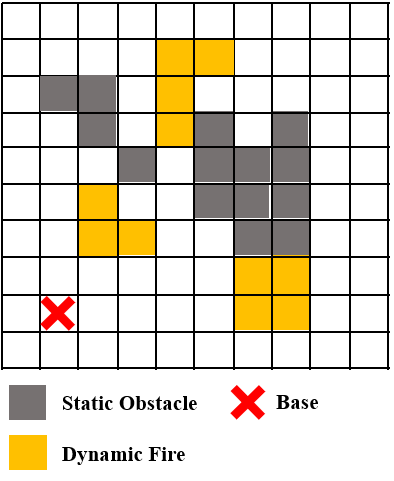
\includegraphics[width = 0.8 \linewidth]{GridPartitionVert}
	\centering
	\caption{2D grid partition of problem location with environmental indicators}
	\label{probpartition}
\end{figure}

 \begin{figure}
	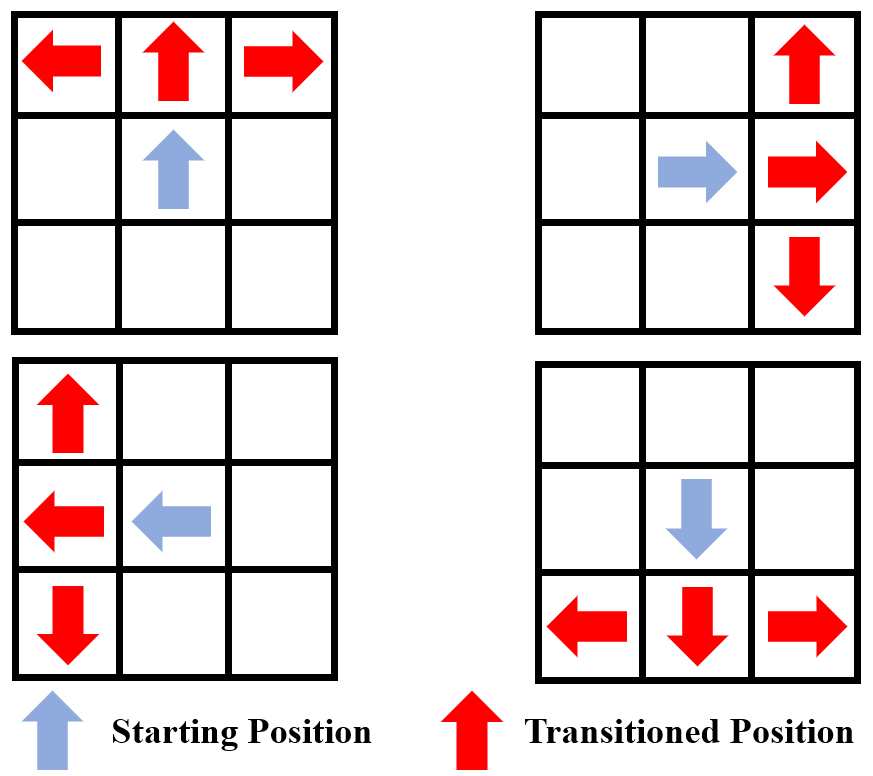
\includegraphics[width = 0.8 \linewidth]{Transitions}
	\centering
	\caption{Possible transitions for UAV within grid given starting orientation and location}
	\label{transitions}
\end{figure}

For the purposes of this paper, suppose that the overall 2D region is partitioned into a granular 10x10 grid (units ignored, density 1), as shown in \ref{probpartition}, with each forested partition (shown as empty) capable of experiencing fire within it. UAVs can transition throughout these partitions in the manner displayed in \ref{transitions} and have the ability to stop within a partition, indicating landing. As such, the states of the UAVs $S$ consist of their position in the grid $s_{p}$ and orientation $s_o \in \{1,2,3,4\}$. Additionally, the UAVs’ states include the water level ($w \in \{4,3,2,1,0\}$), and therefore $S = s_p \cup s_o \cup w$

The fire behaves as described. A partitioned subdivision contains $f$ amount of fuel. As long as the fuel amount sits above $0$, the subdivision can hold a fire. The fire itself varies in intensity, with levels of $Low$, $Medium$, and $High$. A fire will grow in intensity with time, the duration of growth diminishing at each higher level of intensity. Every time a fire grows in intensity, all adjacent partitions that do not currently hold fire and do contain fuel will begin holding fire, starting at the lowest intensity. These rules are detailed further in the \textit{Implementation} section.

Design specifications for each individual UAV are as follows. Each UAV must only drop a fraction of its water supply (transitioning from the current amount to next lowest) when flying over designated fire regions (the amount dropped will result in varying degrees of effectiveness), and each UAV must return to base for replenishing water supplies when $w = 0$. Additionally, the UAVs experience engine problems and must land for prolonged periods of time in the next available region not consumed by fire. Lastly, the UAVs must coordinate when asked, dropping water on the same location just as another UAV does so also. 

The design goal for this problem scenario is to create a high-level autonomous controller to dictate the overall behavior of the fleet for tackling any generic fire situation while maintaining the desired design specifications per UAV and achieving the overarching goal of permanently extinguishing all fires. The open-ended nature of this design goal leaves plenty of flexibility in the remaining environmental design and allows for the exploration of the effectiveness of this paper’s proposed solution.

\subsection{Possible Solution Methods}
To begin, suppose a singular design approach is utilized for tackling this scenario, i.e. one methodology is utilized for achieving the high-level goal and design specifications.

First, attempting to meet all specifications with strong performance towards fighting fires through synthesizing a single controller to dictate the behavior of all the UAVs together would be impractical. As mentioned in the \textit{Introduction}, the arbitrary nature of the fires combined with extensive system variables within the large state space provided creates an infeasible amount of possible permutations. Additionally, further system variables and specifications would need to be added for describing performance metrics and coordination. As discussed later on in this paper (in the \textit{Implementation} section), breaking down the synthesis problem still provided excessive state spaces to explore, and the futility of attempting a singular synthesized solution became readily apparent.

Second, tackling design through an allocation process that manages which UAVs should go to which fires would provide a reasonable approach to managing the control of the fires through what is essentially an allocation of resources. An allocation process based on the one shown in \textcolor{red}{[CITE]} could incorporate a performance function for each UAV that weighs the distance of each fire to the UAV and the fires' intensities and proximity to other fires. The process would allocate each UAV to the fire that maximizes said performance function. On the flip side, though, such an allocation process would not manage information regarding the dynamics of the UAVs, control of their transitions and water levels, and determining when the UAVs should emergency land. An allocation process is well suited for a piece of the problem, but not necessarily the whole scenario.

Lacking on their own, the two methods presented above could combine to meet the desired design specifications for the presented problem scenario. While the combination of these two particular methods is plainly the explored solution for this paper, it is worthwhile to quickly discuss advantages and disadvantages of what is perhaps the more obvious solution method.

Suppose the design was created through a “handcrafted” approach, akin to many designs methods utilized in autonomous systems today \textcolor{red}{(Need examples??)}. Utilization of a path planning algorithm (such as the one used in \textcolor{red}{[d*]}) for sending UAVs to any given destination (i.e. a fire or base) from any starting condition, could be combined with the described top-level allocation process that managed the destinations for all UAVs together. A huge benefit of such an approach is that the dedicated path-planning algorithm could handle a greater variety of dynamic environments than a synthesized controller. On the flip side, depending on the exact path planning algorithm, the path planning may not anticipate and handle obstacles much larger than its scale of operation. Additionally, the described approach could easily be susceptible to programming errors due to the necessity of creating the conditions that dictate other task-oriented operations of the UAV (such as those involving control of the water level, knowing when to land under what conditions, synchronizing with other UAVs, etc.). Furthermore, the syncing behavior for the UAVs might require another method to force such an outcome, or perhaps the allocation process would need to grow to accommodate such a behavior, which would require an understanding of the locations of the UAVs and how their possible transitions could enable synchronization. Evidently, a “handcrafted” approach to the problem would require isolation of all possible behaviors and encoding methods to resolve each, precisely the issue that reactive synthesis aims to avoid.

\section{Proposed Solution Method}
In this paper, we propose a solution method that combines reactive synthesis with allocation. These two methods form a high-level planner and controller that fulfills the design constraints imposed on each UAV and dictates the behavior of each individual UAV as well as their collective maneuvers. \ref{RHAlloc} depicts a conceptual view of the duties that each method fulfills and how each interacts with the other.

 \begin{figure}
	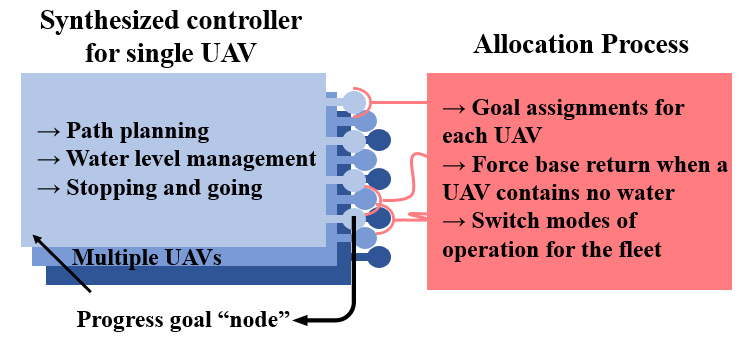
\includegraphics[width = 0.8 \linewidth]{RHandAllocationDesc}
	\centering
	\caption{Diagram of responsibilities and roles for both the synthesized controllers and the allocation process}
	\label{RHAlloc}
\end{figure}


As shown in \ref{RHAlloc}, a common synthesized controller exists for each of the UAVs. This single controller dictates: high-level path planning through the partitioned space; the control of the water level; stopping during perceived engine failure; and synchronization with other UAVs. Each controller also aims to progress to each partitioned region given any arbitrary initial condition. The order of these progress statements, though, are not dictated by the synthesized controller. Instead, the allocation process decides which progress specification any single UAV should pursue. Hence, the allocation process is in charge of: assigning goals for the UAVs; forcing each UAV to return to home when water is depleted; and switch its own internal mode to prioritize different types of firefighting (synchronized fighting vs. non-synchronized fighting).

\section{Implementation}
\subsection{Step I. Synthesis of Controllers in Receding Horizon framework}
For the synthesized controller, the following environmental and system variables for a single UAV were created. The environment consisted of: $StopSignal$, representing whether or not the UAV needs to stop; $Fire$, representing the presence of fire directly beneath the UAV; and $SyncSignal$, representing the UAV’s detection of whether or not a nearby UAV can enter the desired goal location. Hence, the environment $E$ equals ${StopSignal \cup Fire \cup SyncSignal}$. The system consists of $S$ as described in the \textit{Problem Scenario} section. Additional APs $GoalPos_i$ and $Base$ are used for when the UAV enters any specified goal location (indexed with $i$) and the Base location, respectively.

The overall environment specifications for a single UAV are listed as follows. 

\begin{equation}
\varphi_{init}^{e} = \lnot StopSignal \land \lnot Fire
\end{equation}
\begin{equation}
\varphi_{s}^{e} = \{\}
\end{equation}
\begin{equation}
\begin{aligned}
\varphi_{p}^{e} = \always \eventually SyncSignal \land \always \eventually \not StopSignal \land \always \eventually \lnot Fire
\end{aligned}
\end{equation}

The overall system specifications for a single UAV are listed as follows.

\begin{equation}
\varphi_{init}^{s} = \lnot \Phi \land w = 100
\end{equation}
\begin{equation}
\begin{aligned}
\varphi_{s,1}^{s} = \always (StopSignal \land \lnot Fire \rightarrow sys\_actions = "Stop")
\end{aligned}
\end{equation}
\begin{equation}
\begin{aligned}
\varphi_{s,2}^{s} = \always (\lnot ( StopSignal \land \lnot Fire ) \rightarrow sys\_actions = "Go")
\end{aligned}
\end{equation}
\begin{equation}
\begin{aligned}
\varphi_{s,3,i}^{s} = \always ((\lnot ( w = 0 ) \land SyncSignal \land GoalPos_i \land \lnot Base) \rightarrow (w \rightarrow w - 1)
\end{aligned}
\end{equation}
\begin{equation}
\begin{aligned}
\varphi_{s,4,i}^{s} = \always ((\lnot (SyncSignal \land GoalPos_i \land Base) \rightarrow (w \rightarrow w)
\end{aligned}
\end{equation}
\begin{equation}
\begin{aligned}
\varphi_{s,5,i}^{s} = \always ( w = 0 \land SyncSignal \land GoalPos_i \land \lnot Base) \rightarrow (w \rightarrow w )
\end{aligned}
\end{equation}
\begin{equation}
\begin{aligned}
\varphi_{p,i}^{s} = \always \eventually SyncSignal \rightarrow GoalPos_i
\end{aligned}
\end{equation}

 \begin{figure}
	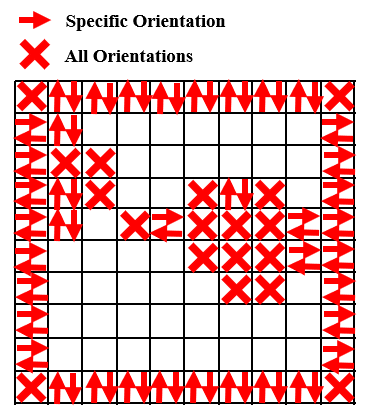
\includegraphics[width = 0.8 \linewidth]{Phi}
	\centering
	\caption{All positions and orientations included in $\Phi$}
	\label{Phi}
\end{figure}

As presented for the system, the initial conditions consist of all possible states except for those consisting of $\Phi$, which consists of the states shown in \label{Phi}. Safety specifications $\varphi_{s,1}^{s}$ and $\varphi_{s,2}^{s}$ dictate the motion of the UAV, with $sys\_actions$ representing whether the UAV should move or stay in the same state. The rest of the safety specifications pertain to how the UAV should control its water levels, such as dropping water over any goal location and refilling when it arrives at base. The set of progress specifications $\varphi_{p,k}^{s}$ (with $k$ indexed through the total sum of possible fire locations) indicate that the UAV should visit all specified locations infinitely often \textit{when the $SyncSignal$ is true}. 

%The environmental initial conditions $\varphi_{init}^{e}$ are the entire possible set. The environmental safety conditions $\varphi_{s,i}^{e}$ are none. The environment progress conditions $\varphi_{p,i}^{e}$ consist of $SyncSignal$ (i.e. each environmental variable will always eventually turn true). The system initial conditions $\varphi_{init}^{s}$ consist of every possible starting location and orientation that does not exist on an obstacle or would lead directly into an obstacle or region edge. Additionally, all $w$ values (system water levels) are included in the possible initial conditions. Transitions are split between action sets titled $“Go”$ (must transition to new position) and sets titled $“Stop”$ (must stay within previous position). The safety specifications of the system $\varphi_{s,i}^{s}$ are listed in Equations Blank.

%\begin{equation}
%\always (StopSignal \land \lnot Fire \rightarrow sys\_actions = "Stop")
%\end{equation}
%
%\begin{equation}
%\always (\lnot ( StopSignal \land \lnot Fire ) \rightarrow sys\_actions = "Go")
%\end{equation}

%\begin{equation}
%\always ((\lnot ( w = 0 ) \land Goal \land GoalPos \lnot Base) \rightarrow (w %\rightarrow w - 1)
%\end{equation}

%\begin{equation}
%\always Base \rightarrow (w \rightarrow 100)
%\end{equation}

%\begin{equation}
%\always ((\lnot (Goal \land GoalPos \land Base) \rightarrow (w \rightarrow w)
%\end{equation}

%\begin{equation}
%\always ( w = 0 \land Goal \land GoalPos \lnot Base) \rightarrow (w \rightarrow w )
%\end{equation}

\begin{figure}
	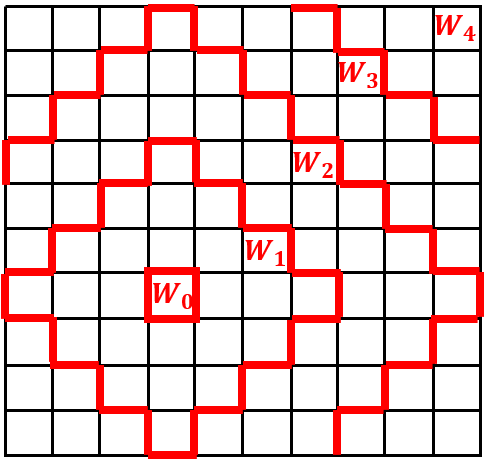
\includegraphics[width = 0.8 \linewidth]{WPartitionPic}
	\centering
	\caption{RH Partitions for Progress Statement Centered on Position (4,4)}
	\label{fig:circuit2}
\end{figure}

Clearly, given any excessively large value of $i$, the total specification would yield a synthesized controller that would first, take an impractical amount of time to generate, and second, create no practical performance with regards to extinguishing fires. From such, though, the RH framework is applied to the synthesized controller, as followed from (CITE). For every progress specification, the partitioned grid is further segmented into subregions $W_j^i$, and example of which is shown in \label{fig:circuit2}. As displayed, the regions are ordered based on their distance from the position that fulfills the particular progress statement.

For each set of regions $W_j^i$, a function $F^i(W_j^i)$ is defined as $F^i(W_j^i)=W_{j-1}^i$, leading the state down the ordered set towards $W_0^i$ and eventually fulfilling the desired progress statement. For each subregion $W_j^i$, an individual GR(1) form is defined as shown previously in ().

TuLiP (CITE) was utilized to realize and synthesize the controllers associated with each region $W_j^i$. On an Intel i5-6500 CPU @ 3.20 GHz processor, this total process, approximately 250 regions $W$, took on the order of 8 hours. On top of the large amount of time to synthesize all of the individual controllers, numerous memory issues came up throughout the process, even with a system limit of 16 GB of RAM.

\subsection{Step II. Dynamic allocation}

In this paper, we propose an efficient method for managing the dynamic allocation of UAVs to fire locations that spread with time. The allocation process considers two paramaters, fire density and proximity of the UAVs to fire locations. Regions with higher fire densities correspond to areas with a higher number of fires concentrated in a region. To partition the map into regions according to their fire densities, the first step in our allocation process is to carry out the K-means $clustering$ $algorithm$ via the Matlab built-in function, $kmeans$. We set this function to use the Manhattan distance as the evaluation index of similarity in order to group fires with similar locations into the same cluster. The $kmeans$ function requires a desired number of clusters, $k$, as input. 

To find the optimal $k_{opt}$, the elbow method is used. Similar work on utilizing the elbow method and other clustering techniques is shown in [X]. In the elbow method, the process iterates through the possible number of clusters, $k$, from 2 to some maximum number of clusters, $K_{max}$, and the sum of square error ($SEE$) for each $k$ is computed. Ideally, we are looking for a value of $k$ that results in clusters that have a low $SEE$. This would lead to fires with high location similarity being assigned to the same cluster. The optimal number of clusters is the value of $k$ at which the second derivative of the average of $SEE(k)$ is maximized. The idea is that the marginal drop in the average $SEE$ as $k$ increases will decrease dramatically for some value of $k$ before it reaches a plateau, hence the ``elbow criterion''. The partition algorithm is summarized in Algorithm I.
\begin{algorithm}
	\caption{Partition algorithm}\label{alg:kMeans}
	\begin{algorithmic}[1]
		\Procedure{clustering}{$K_{max},fireLocs$}
		\State Set $k = 2$
		\While{$k < K_{max}$} 
		\State Compute clusters set $C = kmeans(fireLocs,k)$ 
		\State Compute mean sum of square error with k clusters, $SEE_{avg}(k)$
		\EndWhile
		\State Set optimal $k$, $k_{opt} = k$ that maximizes the second derivative of $SEE_{avg}(k)$
		\State Generate initial cluster centroid positions $C_{init}$
		\State Compute clusters set $C = kmeans(fireLocs,k_{opt},C_{init})$
		\State Assign $fireLocs$ to their corresponding cluster $c \in C$, 
		\State \textbf{return} $C$, fire location assignments
		\EndProcedure
	\end{algorithmic}
\end{algorithm}

Once the map is divided into clusters, the number of UAVs that will be allocated to each cluster is defined by (),
\begin{equation}
N_{alloc}(c) = \ceil[\big]{\rho_{c}/\rho_{tot}\times(N_{tot} - N_{free})},
\end{equation}
where $\rho_{c}$ is the cluster priority calculated as the sum of intensity values of fires that belong to cluster $c$, $\rho_{tot}$ is the sum of intensity values of all fires. $N_{tot}$ is the total number of UAVs and $N_{free}$ is the number of UAVs that are not assigned to a cluster. For each cluster $c$, we assign a subset of UAVs chosen from all available UAVs. This subset of size $N_{alloc}$ is comprised of those UAVs with locations closest to $c$. Once each cluster $c$ has an assigned subset of UAVs, the next step is to decide the fire location belonging to $c$ for each UAV to set as its goal. We have two modes in which UAVs can be assigned to fires, $Sync$ mode and $NonSync$ mode. 

In $Sync$  mode, for each cluster $c$, we loop through each UAV from the assigned subset to $c$ and determine the fire with the minimum cost, proportional to its distance from the UAV, and highest priority, proportional to the fire intensity, according to function $g$ as shown in (). The rest of the UAVs in the loop are assigned to the same fire as the first UAV in the loop.
\begin{equation}
\min_{f\in F} g(f,x) = d_{f}*\norm{x-f} + s_{f}*\norm{g-f} - n_{f}*intensity_{f},
\end{equation}
where $d_{f}$ is a coefficient between 0.0 and 1.0 and is used as an importance weight for the distance between UAV location $x$ and fire $f$ $\in$ $F$. $F$ represents the set of all fire locations in cluster $c$. The coefficient $n_{f}$ represents an importance weight for the fire intensity level, $intensity_{f}$. This coefficient is set as 1.0 - $d_{f}$. Finally, coefficient $s_{f}$ corresponds to the switching penalty of changing an already assigned fire to a different fire, if the assigned fire has not been reached yet. If the UAV reaches its assigned fire, then the minimization is done over all other fires.  

In $NonSync$ mode, for each cluster $c$, we also loop through each UAV from the assigned subset, but only one UAV is assigned to a single fire. The fire is chosen from the set of unassigned fires for each UAV according to (). Each time a fire is assigned, it is removed from the set $F$. 

\subsection{Step III. Simulation}

To test the combination of the allocation process and the synthesized controllers, a simulation was constructed within MATLAB. The primary loop of the simulation incremented per move-set instead of with time, i.e. every action of the environment and reaction of the system occur within what is considered the same move. The environment consisted of the fires in each partition, the intensity of each fire, the number of moves before each fire intensity increased, the amount of fuel left in each partition, and a random engine failure signal that forced UAVs to land.

Variables pertaining to the fire behavior at each level of intensity are displayed in ()

\begin{table}[H]
	\caption{Fire growth behavior}
	\label{table_4}
	\scalebox{0.9}{
		\begin{tabular}{|c||c||c||c|}
			\hline
			Fire Intensity Level & \multicolumn{1}{|p{3cm}|}{\centering Required Number of Moves \\ before Intensity Increase} & \multicolumn{1}{|p{3cm}|}{\centering Fuel Consumption at \\ Intensity Increase} \\ 
			\hline
			1 & 10 & 1 \\ 
			\hline
			2 & 7 & 1 \\
			\hline
			3 & 5 & 1 \\
			\hline
		\end{tabular}
	}
\end{table}

When a fire grew in intensity, it spread to adjacent partitions that contain fuel and no fire, starting new fires at intensity levels of 1. Additionally, if a fire was at intensity level of 3, it would continue to remain at 3.

A feedback loop for enacting the impact of water dropped on fires was also implemented. The amount of water dropped from UAVs into each partition was recorded at each move, and a rule set was followed for changing a partition's fire status from the dropped water. This rule set is displayed in ().

\begin{table}[H]
	\caption{Fire response behavior}
	\label{table_3}
	\scalebox{0.9}{
		\begin{tabular}{|c||c||c||c|}
			\hline
			Fire Intensity Level & \multicolumn{1}{|p{3cm}|}{\centering Amount of Water Dropped \\ (\% of UAV Tank)} & Resulting Fire Intensity\\ 
			\hline
			1 & $\geq$ 80\% & 0 \\ 
			\hline
			1 & $<$ 80\% and $\geq$ 40\% & 0 \\
			\hline
			1 & $<$ 40\% & 0 \\
			\hline
			2 & $\geq$ 80\% & 0 \\
			\hline
			2 & $<$ 80\% and $\geq$ 40\% & 1 \\ 
			\hline
			2 & $<$ 40\% & 1 \\
			\hline
			3 & $\geq$ 80\% & 0 \\
			\hline
			3 & $<$ 80\% and $\geq$ 40\% & 2 \\
			\hline
			3 & $<$ 40\% & 3 \\
			\hline
		\end{tabular}
	}
\end{table}

The response of any fire to water dropped was constructed around the possible drop amounts (corresponding to the allowed water level transitions with and without UAV synchronization). Additionally, when water dropped on a fire, the fire update counter restarted at 0 and the fuel level remained as it was before.

The simulation loop structure followed as such:

\begin{algorithm}
	\caption{Simulation Loop}\label{alg:sim}
	\begin{algorithmic}[1]
		\Procedure{SimulationRun}{}
		\State Initialize UAVs locations and fire locations
		\While{Simulation Runs} 
		\State Update fire growth
		\State Allocate UAVs based on fire state
		\State Move UAVs forward through synthesized controllers
		\State Implement feedback changes on fires due to water dropped
		\EndWhile
		\EndProcedure
	\end{algorithmic}
\end{algorithm}

\iffalse
In the estimation process, the state of the system is expressed as a valuation of the state of individual components and uncontrollable contactors. Controllable and uncontrollable contactors are user-defined and remain unchanged throughout the estimation process. Let $X$ be the state of the circuit, modeled as a random variable. First, the circuit is assumed to be in an unknown state $x_{0} \in \Omega$, where $\Omega$ represents the set of all possible states. Let $V = \{(v_{i})_{i\in\{0,...,t\}}\}$, represent the set of actions that can be performed on the controllable contactors. Let $Y$ be the set of sensor measurements, with $y = \mu(v,x) \in Y$ representing the unique outcome of performing action $v$ for a system state $x$. For actions $\{v_{0}, ..., v_{t}\}$ and outcomes $\{y_{0}, ..., y_{t}\}$ observed up until step $t$ are represented by the partial realization $\psi_{t} = \{(v_{i}, y_{i})_{i\in\{0,...,t\}}\}$. The estimation process adaptively gets to the actual state $x_{0}$. Let $D(y,v)$ with $y = \mu(v,x_{0})$ be the set of states that are indistinguishable from $x_{0}$ under action $v$. Let $S_{t}$ = $h(v_{0:t}, x_{0})$ be an extension of this set containing states that produce the same set of outcomes as $x_{0}$ under the same set of actions $\{v_{0}, ..., v_{t}\}$. At each time step $t$ that a new action $v'\not\in\psi_{t}$ is taken, there exists a recursive relation between the two sets of states: 
\begin{equation}h(v_{0:t}\cup\{v'\},x_{0}) = h(v_{0:t}, x_{0})\cap D(\mu(v', x_{0}),v'), \end{equation}
and $S_{t}$ becomes:
\begin{equation}S_{t}=\cap_{i\in\{0,\ldots, t\}}D(\mu(v_{i}, x_{0}), v_{i}). \end{equation}

A strategy $\pi$ is defined as a function of partial realizations to actions where $\pi(\psi_{t}) =  v_{t+1}$. For an initial configuration with $x_{0}$, $v_{0}$ and $y_{0}$, the sequence of decision, measurement and update operations of the estimation process are expressed in Equations (3a)-(3c) respectively:
\begin{subequations}
\begin{align}
v_{i}&=\pi(\psi_{i-1})\\
y_{i}&=\mu(v_{i}, x_{0})\\
\psi_{i}&=\psi_{i-1}\cup(v_{i}, y_{i})
\end{align}
\end{subequations}

The goal is to reduce the uncertainty in the state estimate, thus minimizing the number of indistiguishable states, by performing $k$ $\in \{0, ...,t\}$ actions that maximize the objective function $f$. This function maps the set of actions $A\subseteq V$ under state $x_{0}$ to reward $f(A, x_{0})$, which measures the reduction in uncertainty of $X$ represented by the probability distribution $\mathbb{P}[x]$ through performing $k$ actions:

\begin{equation}
f(v_{0:k}, x_{0})=-\mathbb{P}[S_{k}]=-\sum_{x\in S_{k}}\mathbb{P}[x]. 
\end{equation}

Thus, the estimation will find the strategy $\pi$ that allows the best expected estimate for the state as shown in (4). We denote $|\tilde{V}(\pi,x_{0})| \subseteq V$ the set of all the actions performed under the strategy $\pi$, the state of the system being $x_{0}$.

\begin{equation}
\pi^{\ast}\in\mathop{\arg\max}\limits_{\pi} \mathbb{E}[f(\tilde{V}(\pi, X), X)], 
\end{equation}
subject to $|\tilde{V}(\pi,x)| \leq k$ for all $x$, and with expectation taken with respect to $\mathbb{P}[x]$. A greedy strategy is then used to select, at each 
step $t$, the action $v_{t+1}$ that maximizes the expected one-step gain in uncertainty reduction with respect to all previous actions:
\begin{equation}
v_{t+1}\in \mathop{\arg \max}\limits_{v\in {\tilde{V}}} \mathbb{E}[f(v_{0:t}\cup\{v\}, X)-f(v_{0:t}, X)\vert \psi_{t}].
\end{equation}


The overall goal is to design a strategy the fault detection controller runs to adaptively estimate the discrete state of the circuit by taking actions
(i.e., closing and opening controllable contactors), and then
reading voltage sensor measurements. 

By changing the number and locations of sensors, it may be possible to improve state estimation performance. In the next section, a sensor placement algorithm is proposed to determine the number of sensors and locations with the goal of maximizing the performance of the state estimation method.

%######################
% Given example for this 
% write transitions: Now we are going to describe the and give some theoretical background
%######################

\subsection{Sensor placement} 
% Some of these algorithms are shown to be too computationally demanding and subject to modeling errors.
Two algorithms explored in [11]-[12] for different applications are adapted to address our sensor placement problem. One proposes a combinatorial approach and the other a greedy approach, as shown in [11] and [12] respectively. Both approaches seek to maximize the state estimation ratio. This ratio is computed for a given sensor placement strategy $P$ as follows,
\begin{equation}r(P) = \frac{n_{succ}}{n_{tot}},\end{equation}
where $n_{succ}$ is the number of state configurations for which the state estimation algorithm returns a unique state (i.e. number of successful runs) and $n_{tot}$ is the total number of state configurations. 

The combinatorial algorithm is used as a reference since it considers all possible combinations of the desired number of sensors out of the total available sensors and outputs the combination of sensors that results in the maximum state estimation ratio. Unlike the combinatorial algorithm, the greedy algorithm does not need to consider all possible sensor combinations to achieve the same results, making it a much better candidate for our methodology. We use the ideas in [12] to develop our greedy algorithm and provide a theoretical description of this algorithm below. 
% This approach guarantees finding the optimal solution since it examines all possible sensor placement scenarios.  
% framing the sensor selection problem as an N choose k problem

\subsubsection{Background}
In [12], the problem of sensors and actuators placement is analyzed as a set function optimization problem of the form
\begin{equation}\mathop{\hbox {maximize}}\limits_{P\subseteq L,\ \vert P\vert=k}\quad r(P),\end{equation}
where $L = \{1,...,M\}$ is a finite set and $r: 2^{L} \rightarrow \mathbb{R}$ is a set function. $L$ represents the set of potential locations for the placement of sensors or actuators and $r$ is a metric for how controllable the system is for a given set of placements.
After proving mathematically that $r$ is a monotone increasing submodular function, a greedy heuristic is used to obtain a sub-optimal solution with guaranteed worst-performance bounds [19], [20]. For $r$ to be submodular and monontone increasing, the following equations need to be satisfied respectively:
\begin{equation}r(A\cup\{p\}) -r(A) \geq r(B\cup\{p\}) -r(B),\end{equation}
for all subsets $A$ $\subseteq$ $B$ $\subseteq$ $V$ and all elements $p$ $\notin$ $B$,
\begin{equation}A \subseteq B \Rightarrow r(A) \leq r(B), \end{equation}
for all subsets $A$, $B$ $\subseteq$ $V$.

The greedy algorithm starts with an empty set, $P_{0} \leftarrow \emptyset$, computes the gain $\Delta(a\vert P_{i})=r(P_{i}\cup\{a\}) - r(P_{i})$ for all elements $a\in V\setminus P_{i}$ and adds the element with the highest gain
\begin{equation}P_{i+1}\leftarrow P_{i}\cup\left\{\arg\max_{a}\Delta(a\vert P_{i})\vert a\in L\setminus P_{i}\right\}.\end{equation}
\subsubsection{Implementation}
In our implementation of the greedy algorithm, we set the function $r$ in (9) to be the state estimation ratio. Since this function is submodular monotone increasing, the greedy algorithm will provide sub-optimality guarantees as shown in [12]. Thus, the greedy algorithm obtains a sensor placement strategy by making a sequence of choices. At each step $i$, it assumes that $i$ sensor locations are fixed and makes a greedy choice where to place the $(i + 1)$-th sensor. The sensor location added at each step is the one that maximizes the gain in the estimation ratio. The pseudocode for the greedy estimation algorithm is shown in Algorithm 1.
% We expect the combinatorial one to provide an optimal solution but be too computationally demanding and the greedy one to provide sub-optimal gurantees but perform much faster.
%\subsubsection{Implementation}
% Similar to work presented in [12] for wireless sensor networks and [14] for dynamical networks, we adapted these ideas to develop two methods for sensor placement for a given circuit. Both methods seek to select sensors that will maximize the performance of the state estimation algorithm. We quantify this performance by computing a function of the results obtained by the state estimation algorithm when run for all possible system states with the given sensor placement. This function is calculated as the ratio of the number of state configurations for which the state estimation algorithm returns a unique state (i.e. number of successful runs) over the total number of configurations. We will refer to this function as the estimation success ratio throughout the paper. 
% The first method implemented is the combinatorial method based on the combinatorial approach n choose k. This method selects the combination of sensors that results in the maximum estimation success ratio as the sensor placement strategy. The pseudocode for the combinatorial method is as follows.
% \begin{algorithm}
% \caption{Combinatorial Sensor Placement Algorithm}
% \begin{algorithmic}[1]
% \Procedure{maxSelection}{$n,k$,sensors}
% \State Loop through the set of all possible combinations of the sensors,\begin{align*}
% s = {n \choose k}
% \end{align*}  where n is the total number of sensors and k is the number of required sensors
% \State For each combination in s, attach the chosen sensors to the circuit configuration
% \State Load in the database of states mapped to measurements for the modified configuration
% \State Calculate the estimation success ratio and store it in an array
% \State Select the combination of sensors for which the estimation success ratio is maximum
% \State \textbf{return} sensor placement strategy
% \EndProcedure
% \end{algorithmic}
% \end{algorithm}
% Next we have the greedy method which obtains a sensor placement by making a sequence of choices. At each step i, it assumes that i sensor locations are fixed and makes a greedy choice where to place the (i + 1)-th sensor. The sensor location added at each step is the one that maximizes the gain in the estimation success ratio. Hence, this method is an adaptation of the greedy heuristic with sub-optimality guarantees in [14]. It is important to note that the estimation success ratio acts as the submodular monotone increasing function in our implementation. The pseudocode for the greedy estimation success algorithm is shown in Algorithm 2.
\begin{algorithm}
  \caption{Greedy Sensor Placement Algorithm}\label{alg:greedy}
  \begin{algorithmic}[1]
    \Procedure{greedySelection}{$r,p,e,k,n$}
      \State Initialize the maximum estimation ratio $r$ to 0.0
      \State Initialize the desired ratio $p$ to 0.8
      \State Initialize the number of chosen sensors $n$ to 0
      \State Initialize the sensor placement strategy $S$ to $\{\}$
      \While{$r < p$ and $n < k$} 
      	\For{each sensor location $Li$ in Fig. 2} 
			\If{$Li$ has not been selected already}
				\State Load the measurements database for $S$ $\cup$ $Li$
				\State Calculate the estimation ratio $e$
				\If{$r < e$}
					\State $r = e$
					\State $Lchosen = Li$
				\EndIf
			\EndIf
		\EndFor
		\State $S$ $=$ $S$ $\cup$ $Lchosen$ 
		\State $n = n + 1$
      \EndWhile\label{euclidendwhile}
    \State \textbf{return} sensor placement strategy
    \EndProcedure
  \end{algorithmic}
\end{algorithm}
% \State Place the sensors in the circuit available locations as shown in Fig. 2
% \begin{algorithm}
% \caption{Greedy Sensor Placement Algorithm}\label{alg:greedy}
% \begin{algorithmic}[1]
% \Procedure{greedySelection}{$n,k$,sensors}
% \State Initialize the maximum success ratio to 0.0
% \State Attach the sensors to the locations chosen by the sensor placement strategy from the available sensor locations as shown in Fig. 2
% \State Loop through each of the unselected available sensors and attach it to the circuit 
% \State Load in the database of inverse mapping from sensor measurements to compatible states of the circuit for the modified configuration  
% \State Calculate the success ratio, if it is greater than the current maximum success ratio, set it as the maximum success ratio 
% \State Go to the next sensor and repeat from step 4
% \State Add the chosen sensor that corresponds to the maximum success ratio to the sensor placement strategy
% \State Go back to step 2 and repeat from there until k sensors are selected or the state estimation success percentage threshold is satisfied
% \State \textbf{return} sensor placement strategy
% \EndProcedure
% \end{algorithmic}
% \end{algorithm}

Once the sensors are connected in the locations determined by the strategy, the off-line step of the methodology is completed. Using this sensor placement, state estimation can be periodically run to monitor for faults. The state estimates obtained are passed to the controller synthesis in order to proceed with fault restoration if the state estimate reveals a fault in any component of the system. Fault restoration will generate actions to reroute power to ensure safe operation in the system. These actions are dictated by a control protocol built by verification and synthesis techniques described below.
%######################
% write transitions: Now we are going to describe the and give some theoretical background
%######################
\subsection{Controller Synthesis}
As shown in [13], [14] and [15], we can translate system requirements written in English to a temporal logic specification language (e.g., Linear Temporal Logic). These specifications are used to define correct behaviors of a system. Using this approach, a correct-by-construction controller can be designed to reconfigure the electrical power system to address different system failure scenarios. Whenever a system component becomes faulty, this would characterize a specific environment scenario and the controller is designed to react to it according to some high-level specifications. The output of the controller will be a different sequence of actions in each execution since the environment may be different. This captures the reactive nature of the controller. In [13], two approaches for designing the controller are the centralized and the distributed approach as described below.
 % And a controller can be designed to take actions to guarantee these behaviors even in the presence of system failures. The building block of LTL is the atomic proposition. An atomic proposition is a statement on a valuation of system variables that has a unique truth value (True or False) for a given value. 
\subsubsection{Centralized synthesis}
In order to design the controller, we first define the system model. The system variables are classified into sets of environment variables $E$ and controlled variables $P$. Let $s = (e,p) \in dom(E) \times dom(P)$ be the state of the system. Consider an LTL specification $\varphi$ of assume-guarantee form,
\begin{equation}\varphi= \varphi_{e} \rightarrow \varphi_{s},\end{equation} where $\varphi_{e}$ characterizes the assumptions on the environment and $\varphi_{s}$ characterizes the system requirements. The synthesis problem
is then concerned with constructing a controller strategy which chooses
the action on the controlled variables based on the state
sequence so far and the behavior of the environment so
that the system satisfies the system requirements as
long as the environment assumptions are satisfied.

The synthesis problem can be viewed as a two player
game between an environment that attempts to falsify the
specification and a controlled plant that tries to satisfy it. The formula $\varphi$ is true if $\varphi_{s}$ is true, and the system specifications are satisfied. When $\varphi_{e}$ is false, i.e. the environment is inadmissible, the synthesis problem becomes unrealizable and there is no guarantee about the behavior of the system. To obtain LTL formulas, a set of atomic propositions needs to be defined. Any atomic proposition that belongs to this set is an LTL formula. The LTL formulas can express a wide range of system specifications regarding safety, performance, and reliability of the system.
The LTL specifications are then transformed into General Reactivity of Rank 1, GR(1), specifications. It has been shown that realizability and synthesis problems for GR(1) specifications can be solved efficiently in polynomial time and GR(1) is expressive enough to provide complete specifications of many designs [17]. GR(1) is explored in depth in [16]. Thus, both $\varphi_{e}$ and $\varphi_{s}$ have the following structure: 
\begin{equation}
\varphi_{e} = \varphi^{e}_{i} \aand \varphi^{e}_{t} \aand \varphi^{e}_{g}; \enspace
\varphi_{s} = \varphi^{s}_{i} \aand \varphi^{s}_{t} \aand \varphi^{s}_{g},
\end{equation}
where $\varphi^{e}_{i}$, $\varphi^{s}_{i}$ are the initial values for the environment and controlled variables, $\varphi^{e}_{t}$, $\varphi^{s}_{t}$ represent the evolution of the state of the system, and $\varphi^{e}_{g}$, $\varphi^{s}_{g}$ represent goal assumptions for the environment and desired goal specifications for the system. 

The GR(1) specifications are then passed to the synthesizer available in the temporal logic planning (TuLiP) toolbox. For a thorough description of this tool, see [18]. The synthesizer returns a finite-state machine in which states are valuations of environment and controlled variables and transitions are actions that the controller can take to reach a desired state.

When a controller has access to all environment and controlled variables, it functions as a centralized controller. As the number of components increases, the computational complexity can increase significantly. In order to address this and other issues such as system robustness and resilience to failure, a distributed controller strategy is also considered.

\subsubsection{Distributed synthesis}
By using a distributed controller, the system is divided into subsystems and a local controller is synthesized for each one of them. Thus, the synthesis task is divided into smaller subproblems and the computational complexity of the problem is reduced. Also, the distribution of power can be controlled and reestablished for each subcomponent of the system without affecting other subcomponents, leading to a more robust and resilient system. 

Synthesizing a local controller requires the decomposition of global specifications into local specifications. For instance, let a system $SYS$ be decomposed into $SYS_{1}$ and $SYS_{2}$. For $i$ = 1,2, let $E_{i}$ and $P_{i}$ be the environment variables and controlled variables for $SYS_{i}$ such that $P_{1}$ $\cup$ $P_{2}$ = $P$ and $P_{1}$ $\cap$ $P_{2}$ = $\emptyset$. The overall environment assumptions $\varphi_{e}$ and system guarantees $\varphi_{s}$ are distributed into the two systems ${SYS}_{1}$ and ${SYS}_{2}$. Let $\varphi_{e_{1}}$ and $\varphi_{e_{2}}$ be LTL formulas containing variables in $E_{1}$ and $E_{2}$, respectively. Let $\varphi_{s_{1}}$ and $\varphi_{s_{2}}$ be formulas in terms of $E_{1}$ $\cup$ $P_{1}$ and $E_{2}$ $\cup$ $P_{2}$, respectively. Then, as long as the following conditions are satisfied, the distributed control protocol will satisfy the global specifications:
\begin{enumerate}
\item any sequence of actions from the environment that satisfies $\varphi_{e}$ also satisfies ($\varphi_{e_{1}}$ $\land$ $\varphi_{e_{2}}$),
\item any sequence of actions of the system that satisfies ($\varphi_{s_{1}}$ $\land$ $\varphi_{s_{2}}$) also satisfies $\varphi_{s}$, and,
\item there exists two control protocols that realize the local specifications ($\varphi_{e_{1}}$ $\longrightarrow$ $\varphi_{s_{1}}$) and ($\varphi_{e_{2}}$ $\longrightarrow$ $\varphi_{s_{2}}$).
\end{enumerate}
% The interaction between subsystems may be needed for the synthesis problem to become realizable and this can be done through an extra set of local guarantees that interact with each subsystem. For example, let $SYS_{1}$ have an extra set of local guarantees $\phi_{1}$ that interact with $SYS_{2}$ as environment assumptions $\phi_{1}^'$, while $\phi_{2}$ are the local guarantees for $SYS_{2}$ that act as environment assumptions $\phi_{2}^'$ to $SYS_{1}$.
Additional information exchange between subsystems may be needed to make sure these conditions are satisfied. This can be done through an extra set of local guarantees that interact with other subsystems. For example, let $S_{1}$ have an extra set of local guarantees $\phi_{1}$ that interact with $S_{2}$ as environment assumptions denoted as $\phi^\prime_{1}$, while $\phi_{2}$ are the local guarantees provided by $S_{2}$ that interact with $S_{1}$ as environment assumptions denoted as $\phi^\prime_{2}$. Thus, if the local specifications hold, then the global specification $\varphi_{e}$ $\longrightarrow$ $\varphi_{s}$ is realizable as shown in .
\begin{equation}
\phi^\prime_{2} \land \varphi_{e_{1}} \longrightarrow \varphi_{s_{1}} \land \phi_{1}, 
\end{equation}
\begin{equation}
\phi^\prime_{1} \land \varphi_{e_{2}} \longrightarrow \varphi_{s_{2}} \land \phi_{2}.
\end{equation}
\section{Test on a simple circuit}
In this section, we give implementation details on applying the system methodology to the circuit topology shown in Fig. 2.
% some typical aircraft electric power system topologies. In order to reduce online computation, the inverse mapping from sensor measurements to compatible states of the circuit is conducted offline. Additionally, we propose some abstraction rules to reduce the size of the circuit as well as computation time.
% We run the two sensor placement algorithms for the circuit in Fig. 2. 
This circuit topology consists of basic high-voltage AC components: two generators G0-G1 and two AC buses B1-B2, DC components: two rectifier units RU1-RU2 and two DC buses B3-B4, and contactors C1-C8. A discrete model for the circuit is chosen in order to make the integration with the controller synthesis method easier. In this model, generators and rectifier units can be in three states: offline (0), healthy (1) and unhealthy (2). Contactors can be in two states: open (0) and closed (1). Buses can be in two states: healthy (1) and unhealthy (0). Possible values for sensors healthy (1) and unhealthy (0) as well. Component variables and status variables are distinguished by upper and lower cases, e.g., the first generator is represented by G0, while its status is represented by $g_{0}$. 
%\begin{figure}
%  \includegraphics[width = 0.55 \linewidth]{circuit}
%  \centering
%  \caption{A single-line diagram of a simple circuit with AC components and DC components.}
%  \label{fig:circuit}
%\end{figure}
\subsection{Sensor Placement Results}
The first step of the implementation is to generate the databases of the inverse mappings from sensor measurements to compatible states of the circuit for all possible sensor placement configurations. For example, for a given sensor placement configuration, if a sensor were placed at L0, then the database reads a 0 for a fault at G0. Up to 8 voltage sensors can be placed in the circuit. Components (G1;G2;RU1;RU2;C2;C8) are set as uncontrollable and (C1;C3;C4;C5;C6;C7) as controllable. 
% Then, the state estimation algorithm is run for each sensor placement configuration. 
Using the databases obtained for each sensor placement configuration, we can execute the sensor placement algorithms which require the estimation ratio. For performance comparison, we use two versions of the state estimation algorithm to compute this ratio. In one version, the algorithm uses the full greedy strategy in which all possible configurations of the circuit components are simulated systematically as shown in Tables I and III. In the other version, the algorithm uses the reduced greedy strategy in which the initial configuration for the controlled components is fixed as shown in Tables II and IV. 
%The only difference between these two versions is the number of configurations used to calculate the estimation ratio. 
From the results obtained, we can conclude that the performance of the reduced version is better without compromising the accuracy of state estimates. 

For the state estimation step, the greedy strategy is run with a horizon length of k = 6, the number of actions allowed. The status of all sensors is set to healthy. Both sensor placement algorithms were run in Python 2.7 on a 2.3 GHz Intel Core i7 64 bits CPU. The results are shown in Tables I-IV for various numbers of sensors. From these results, we can observe that the sensors selected by each sensor placement algorithm vary, but the same ratio is achieved. For both sensor placement algorithms, the maximum estimation ratio reached was 0.80. This result is the same as the one obtained after placing all available sensors in the system and running the state estimation by brute force method (i.e. where all possible configurations and actions are tested). Thus, for the given circuit set up, the state estimation algorithm can only uniquely identify the state in 80 percent of all possible states. 

To improve this percentage, we consider changing the topology of the circuit. For instance, some uncontrollable contactors are set to be controllable. When contactor C2 is set to be controllable and sensor locations L5 and L6 are chosen, an estimation ratio of 1 is obtained. Allowing more contactors to be controllable improves the estimation ratio as shown in Table V. This happens because the dynamic estimation process has access to a wider range of possible actions that it can take and consequently can gather more information about the state. 
\begin{table}[H]
\caption{Sensor Placement Strategy obtained by the Combinatorial Method with the full version of the adaptive greedy strategy}
\label{table_1}
\scalebox{0.8}{
\begin{tabular}{|c||c||c||c|}
\hline
No of Sensors & Sensor Locations Selected & Estimation Ratio & Execution Time (s) \\ 
\hline
1 & {L7} & 0.14 & 190.17 \\
\hline
2 & {L6, L7} & 0.39 & 871.35 \\
\hline
3 & {L3, L6, L7} & 0.76 & 2203.25  \\
\hline
4 & {L2, L3, L6, L7} & 0.80 &  3134.83 \\
\hline
5 & {L5, L2, L3, L6, L7} & 0.80 & 2657.65 \\
\hline
6 & {L4, L5, L2, L3, L6, L7} & 0.80 & 1396.82 \\
\hline
\end{tabular}
}
\end{table}
\begin{table}[H]
\caption{Sensor Placement Strategy obtained by the Combinatorial Method with the reduced version of the adaptive greedy strategy}
\label{table_2}
\scalebox{0.8}{
\begin{tabular}{|c||c||c||c|}
\hline
No of Sensors & Sensor Locations Selected & Estimation Ratio & Execution Time (s) \\ 
\hline
1 & L7 & 0.14 & 30.25 \\ 
\hline
2 & {L6, L7} & 0.39 & 177.64 \\
\hline
3 & {L3, L6, L7} & 0.76 &  499.19 \\
\hline
4 & {L2, L3, L6, L7} & 0.80 &  804.99 \\
\hline
5 & {L5, L2, L3, L6, L7} & 0.80 & 787.45 \\
\hline
6 & {L4, L5, L2, L3, L6, L7} & 0.80 & 432.88 \\
\hline
\end{tabular}
}
\end{table}
\begin{table}[H]
\caption{Sensor Placement Strategy obtained by the Greedy Method with the full version of the adaptive greedy strategy}
\label{table_3}
\scalebox{0.8}{
\begin{tabular}{|c||c||c||c|}
\hline
No of Sensors & Sensor Locations Selected & Estimation Ratio & Execution Time (s) \\ 
\hline
1 & L6 & 0.14 & 173.68 \\ 
\hline
2 & {L6, L1} & 0.39 & 393.92 \\
\hline
3 & {L6, L1, L5} & 0.76 &  616.69 \\
\hline
4 & {L6, L1, L5, L2} & 0.80 &  773.29 \\
\hline
5 & {L6, L1, L5, L2, L7} & 0.80 & 908.26 \\
\hline
6 & {L6, L1, L5, L2, L7, L3} & 0.80 & 432.88 \\
\hline
\end{tabular}
}
\end{table}
\begin{table}[H]
\caption{Sensor Placement Strategy obtained by the Greedy Method with the reduced version of the adaptive greedy strategy}
\label{table_4}
\scalebox{0.8}{
\begin{tabular}{|c||c||c||c|}
\hline
No of Sensors & Sensor Locations Selected & Estimation Ratio & Execution Time (s) \\ 
\hline
1 & L6 & 0.14 & 17.88 \\ 
\hline
2 & {L6, L1} & 0.39 & 51.59 \\
\hline
3 & {L6, L1, L5} & 0.76 &  89.72 \\
\hline
4 & {L6, L1, L5, L2} & 0.80 &  131.48 \\
\hline
5 & {L6, L1, L5, L2, L7} & 0.80 & 177.47 \\
\hline
6 & {L6, L1, L5, L2, L7, L3} & 0.80 & 251.35 \\
\hline
\end{tabular}
}
\end{table}
\begin{table}[H]
\caption{Sensor Placement Strategy obtained by the Greedy Method for various contactor configurations}
\label{table_5}
\scalebox{0.79}{
\begin{tabular}{|c||c||c||c|}
\hline
Controllable Contactors & Uncontrollable Contactors & Sensors Selected & Estimation Ratio \\ 
\hline
C1 & {C2, C3, C4, C7, C8} & {L7, L6, L1, L0} & 0.0425\\ 
\hline
{C1, C2} & {C3, C4, C7, C8} & {L7, L6, L1, L0} & 0.0825\\
\hline
{C1, C2, C3} & {C4, C7, C8} & {L7, L6, L1, L0} & 0.205\\
\hline
{C1, C2, C3, C7} & {C4, C8} & {L7, L6, L1, L0} & 0.800\\
\hline
{C1, C2, C3, C7, C8} & {C4} & {L7, L6, L1, L0} & 1.000\\
\hline
\end{tabular}
}
\end{table}
While both sensor placement algorithms obtain the same success ratio, the greedy algorithm performs about twice as fast as the combinatorial algorithm. In additon, the greedy algorithm is well-suited for addressing the problem of selecting a required number of sensors and finding the minimum number of sensors that would satisfy an estimation ratio. Thus, we can conclude that the greedy algorithm is better overall.

With the greedy algorithm as the chosen approach, we proceeded to test it further for a scenario in which selected sensors become unhealthy. In this scenario, the greedy algorithm can be run again with new databases. These databases are obtained by simulating erroneous sensor readings corresponding to unhealthy sensors. For example, if an unhealthy sensor were placed at $L_{0}$, then the database reads a 1 for a fault at G0. In this simulation, contactors (C1;C2;C3;C7;C8) are controllable and contactor C4 is uncontrollable. 

Given an estimation ratio of 0.6, the greedy algorithm can output a new sensor placement strategy once sensors become unhealthy. We test this for a given sensor placement in which sensor locations L6 and L7 are initially selected. The results we obtain are as follows. When the sensor placed at L7 becomes unhealthy, the new sensor placement strategy adds a sensor at L5 in order to achieve a ratio of 0.6. If instead sensor at L6 becomes unhealthy, the new sensor placement strategy adds sensors at locations L4 and L5 in order to obtain the same ratio. From these results, we can observe that some sensor locations are more informative than others and additional healthy sensors are needed in order to meet the given threshold.  
% In Table VI, the new sensor placement strategy is shown for various cases of unhealthy sensors. The greedy algorithm outputs a new sensor placement strategy that aims to satisfy a given threshold of 0.6, but in some cases, this threshold is not achievable. For example, for the case in which sensors S6 and S7 become unhealthy, the maximum attainable success ratio is 0.54. 
% After initially selecting sensors S6 and S7, S7 becomes unhealthy
% \begin{table}[H]
% \caption{Sensor Placement Strategy obtained by the Greedy Method with unhealthy sensors }
% \label{table_6}
% \scalebox{0.77}{
% \begin{tabular}{|c||c||c||c|}
% \hline
% Sensors Initially Selected & Unhealthy sensors & Sensors Newly Selected & Threshold Obtained\\ 
% \hline
% S7, S6 & S7 & S6, S5 & 0.6\\ 
% \hline
% {S7, S6} & S6 & S7, S5, S4 & 0.6\\
% \hline
% {S7, S6} & S6, S7 & S5, S4 &  0.54  \\
% \hline
% \end{tabular}
% }
% \end{table}

\subsection{Fault Detection and Fault Restoration Results}
After connecting sensors to locations L4-L7 in the circuit and setting C4 as the controllable variable as determined by the sensor placement strategy for Fig. 2 in Table V, we proceed to implement the second step of the methodology in real-time. First, the state estimation algorithm is run for the circuit with a fixed fault configuration. The resulting state estimate is then passed to the controller synthesis method. 

In order to run the controller synthesis method, we specify the system variables, assumptions on admissible environments and the desired system specifications for the circuit in Fig. 2. The circuit is modeled as a system with environment variables ($g_{0}$;$g_{1}$;$ru_{1}$;$ru_{2}$) for the generators and rectifier units, controlled variables ($c_{1}$-$c_{8}$) for the contactors, and dependent variables ($b_{1}$-$b_{4}$) for the buses. The overall goal of this method is to reconfigure the controlled variables so that power will be delivered to buses and guarantee the following system specifications:

{\bf Environment Assumption:} At least one generator and rectifier unit is always healthy. Also we assume that once a
generator becomes unhealthy, it will remain unhealthy. The specifications to accomplish this are:
\begin{equation}
\always \{(g_{0} = 1) \oor (g_{1} = 1)\},
\end{equation}
\begin{equation}
\always \{(ru_{1} = 1) \oor (ru_{2} = 1)\},
\end{equation}
\begin{equation}
\always \bigwedge_{i = 0}^{1} \{ (g_{i} = 0) \longrightarrow (\next (g_{i} = 0))\}.
\end{equation}

{\bf Unhealthy Sources:} All neighboring contactors to generators and rectifier units that become unhealthy should be set to open. Set of neighboring contactors to generators are $\mathit{N}$(G0) = C1 and $\mathit{N}$(G1) = C2. Neighboring contactors to rectifier units are $\mathit{N}$(RU1) = \{C4, C6\} and $\mathit{N}$(RU2) = \{C5, C7\}. For example, if generator G0 becomes unhealthy, contactor C1 will be set to open. In this instance, the specification for G0 is:
\begin{equation}
\always \{(g_{0} = 0) \longrightarrow (c_{1} = 0)\}.
\end{equation}


{\bf No Paralleling of AC Sources:} In Fig. 2 there is one generator pair \{G0,G1\}. We avoid instances of paralleling ac sources. For example, a live path for the pair {G1,G2} exists if contactors C1, C2 and C3 are all closed. The specification to disallow paralleling of AC sources is:
\begin{equation}
\always \lnot \{c_{1} = 1 \aand c_{2} = 1 \aand c_{3} = 1\}.
\end{equation}

{\bf Power Status of Buses}: A bus will be powered if a live path exists between itself and a generator. A DC bus will be powered if it is connected to a healthy rectifier unit and a live path exists between itself and a powered AC bus. Otherwise, the bus will be unpowered. For instance, the specifications for AC bus B1 and DC bus B6 to be powered are:
\begin{equation}
\always \{(c_{1} = 1 \aand g_{0} = 1) \longrightarrow (b_{1} = 1))\},
\end{equation}
\begin{equation}
\begin{aligned}
\always \{(g_{1} = 1 \aand c_{2} = 1 \aand b_{2} = 1 \aand c_{3} = 1) \\ \longrightarrow (b_{1} = 1)\},
\end{aligned}
\end{equation}
\begin{equation}
\begin{aligned}
\always \{(b_{1} = 1 \aand c_{4} = 1 \aand ru_{1} = 1 \aand c_{6} = 1) \\ \longrightarrow (b_{3} = 1))\},
\end{aligned}
\end{equation}
\begin{equation}
\begin{aligned}
% \begin{split}
\always \{(b_{2} = 1 \aand c_{5} = 1 \aand ru_{2} = 1 \aand c_{7} = 1 \\ \aand b_{4} = 1 \aand c_{8} = 1) \longrightarrow (b_{3} = 1)\}.
% \end{split}
\end{aligned}
\end{equation}

{\bf Essential Buses}: Another specification we consider is that buses B1 and B2 be connected to safety-critical loads, and can be unpowered for no longer than two time steps. Each increment of the clock variable $\theta_{B_{1}}$ and $\theta_{B_{2}}$ represents one time step $\delta$=1. Clock variables function as counter variables and are either increased by 1 or reset to 0 at each step of the execution.

If bus status B1 is unpowered, then at the next time step, clock $\theta_{B_{1}}$ increments by one:
\begin{equation}\tag{10}
\always \{(b_{1} = 0) \longrightarrow (\next \theta_{B_{1}} = \theta_{B_{1}} + 1)\}.
\end{equation}

If bus status B1 is powered, then at the next time step, reset clock $\theta_{B_{1}}$ to zero:
\begin{equation}\tag{11}
\always \{(b_{1} = 1) \longrightarrow (\next \theta_{B_{1}} = 0)\}.
\end{equation}

To ensure that the status of B1 is never unpowered for more than two steps, we have:
\begin{equation}\tag{12}
\always \{\theta_{B_{1}} \leq 2\}.
\end{equation}

We also require that all DC buses must always remain powered by:
\begin{equation}\tag{13}
\always \{b_{3} = 1 \aand b_{4} = 1\}.
\end{equation}


We now turn to define the initial, transition, and goal values for the synthesis in GR(1) form: 
\begin{equation}\tag{14}
\varphi^{e}_{i} = \bigwedge_{i = 0}^{1} \{ (g_{i} = 1), (r_{i} = 1) \}
\end{equation}
\begin{equation}\tag{15}
\varphi^{s}_{i} = \bigwedge_{i = 1, i \neq 3}^{8} \{ (c_{i} = 0) \}
\end{equation}
\begin{equation}\tag{16}
\varphi^{e}_{t} = \vee_{i = 0}^{1} \{ (\next \lnot g_{i}), (\next \lnot r_{i}) \}
\end{equation}
\begin{equation}\tag{14}
\varphi^{e}_{g} = \always \eventually (True)
\end{equation}
\begin{equation}\tag{15}
\varphi^{s}_{g} = \always \eventually (True)
\end{equation}

In the following simulation, we use the centralized controller design. The synthesis method is initiated with the following fault configuration: G0 = 0, G1 = 1, RU1 = 1, RU2 = 0, C2 = 0, C7 = 1. After running the state estimation algorithm with the reduced version of the greedy strategy, a state esimate is obtained in 6.48s. Then, the controller synthesis is run with the specifications and variables set as described above. Processing the specifications and obtaining the controller strategy took 0.58s. In this simulation, a centralized approach is used since the controller has access to all system variables.

In Fig. 3 - 5, we show a simulation trace for the reactive controller. The controller determines which adjacent contactors should be closed to allow power to flow from a healthy component into the components that connect to it or set to open to prevent power flow in from failing components. Assume that at time t = 0, all components of the circuit are in a healthy state as shown in Fig. 3. At time t = 1, G0 and RU2 become unhealthy. The controller then outputs a sequence of actions that reconfigure the circuit by opening contactors C2, C5 and C7 and closing contactor C3 as shown in Fig. 4. Then at time t = 2, G1 and RU1 become unhealthy and the controller reacts by opening contactors C2, C4 and C6 and closing contactor C3 as shown in Fig. 5. 

%\begin{figure}
%  \includegraphics[width = 0.6 \linewidth]{simulation0}
%  \centering
%  \caption{State at t = 0, G0 and RU2 are healthy. Initial configuration.}
%  \label{fig:sim0}
%\end{figure}

%\begin{figure}
%  \includegraphics[width = 0.6 \linewidth]{simulation1}
%  \centering
%  \caption{State at t = 1, G0 and RU2 become unhealthy (shaded) and the controller opens C1, C5 and C7. It also closes C3 to mantain B1 powered.}
%  \label{fig:sim1}
%\end{figure}

%\begin{figure}
%  \includegraphics[width = 0.6 \linewidth]{simulation2}
%  \centering
%  \caption{State at t = 2, G1 and RU1 become unhealthy (shaded) and the controller opens C2, C4 and C6. It also closes C3 to mantain B2 powered.}
%  \label{fig:sim2}
%\end{figure}


\section{Case Study on a Large Circuit}

In this section, we test the scalability and feasibility of the proposed methodology as we examine a large circuit topology shown in Fig. 6. All three algorithms of the methodology are performed on this circuit using a centralized approach and a distributed approach. First, a description of the circuit topology is presented followed by the results obtained from applying the methodology to the circuit. 

\subsection{Circuit Topology Description}
At the top of the circuit topoloy are six AC generators G1-G6. An AC bus is connected to each AC generator. There are 8 AC buses in total. The circuit also consists of rectifier units R1-R8, each connected to a DC bus. R1 and R2 connect to the same DC bus. R3 and R4 also share the same DC bus. All other rectifier units connect to one DC bus each. In total, there are 6 DC buses and 33 contactors. From Fig. 6, it can be observed that the circuit topology is symmetric. 
% The AC bus connected to G1 is connected to another AC bus and to rectifier units R1 and R5. Similarly, the AC bus connected to G4 is connected to another AC bus and to rectifier units R4 and R8. The AC buses connected to G2 and G3 are each connected to rectifier units R2 and R3 respectively.
\subsubsection{Environment Variables}

The environment variables consist of all generators G1-G6 and all rectifier units R1-R8. The health statuses for generators and rectifier units can take values of healthy (1) or unhealthy (0). At each step of the simulation, the environment variables can take a status of healthy or unhealthy subject to the assumption that one generator in the set: \{G1, G2, G5\} and one generator in the set: \{G3, G4, G6\} remain healthy. A similar assumption is put into place for rectifier units, at least one rectifier in the set: \{R1, R2, R5, R6\} and one rectifier in the set: \{R3, R4, R7, R8\} remain healthy. We impose these assumptions when decomposing the circuit so that local specifications can be satisfied in the right side of the circuit as well as in the left side. 

\subsubsection{Controlled Variables}
The controlled variables consist of all contactors C1-C33. Contactors can each take values of open (0) or closed (1). All contactors are assumed to be directly controlled without delays. AC and DC buses are considered as dependent variables since their statuses can be either powered (1) or unpowered (0) depending on the status of neighboring contactors, rectifier units and generators.
%\begin{figure}
 % \includegraphics[width = 1.00 \linewidth]{EntireCircuit}
%  \centering
%  \caption{A circuit topology diagram. There are 6 generators connected to AC buses. There are 8 rectifier units that convert power from AC to DC, and are connected to DC buses. A distributed design decomposition is shown using dashed rectangles. Components enclosed within the dashed rectangles are controlled by their own respective controllers and are given their own sensor placement strategies in the distributed approach. The dashed arrow represents information flow, in the form of a health status variable, directed from subcomponent A to subcomponent B. The solid arrow represents the physical transfer of power from subcomponent B to subcomponent A.}
%  \label{fig:circuit2}
%  \vspace{4mm}
%  \includegraphics[width = 0.81 \linewidth]{componentC}
%  \centering
%  \caption{Subcomponent C of the circuit topology diagram shown in Fig. 6 that connects to subcomponent A. The complete diagram includes subcomponent C and its mirror image, subcomponent D, which is% connected to subcomponent B, the mirror image of subcomponent A.}
%  \label{fig:circuit2}
%\end{figure}
%\begin{figure}
%  
%\end{figure}

% \begin{figure}
%   \includegraphics[width = 0.8 \linewidth]{componentC}
%   \centering
%   \caption{A subcomponent of the circuit topology diagram shown in Figure 6 that connects to subcomponent A. The complete diagram includes this subcomponent and its mirror image, subcomponent D which is connected to subcomponent B.}
%   \label{fig:circuit2}
% \end{figure}

\subsection{Centralized approach}
A system model with environment variables $E$ and system variables $P$, including controlled and dependent variables, is used to represent the circuit. Given environment assumptions $\varphi_{e}$ as in (10)-(12) and system assumptions $\varphi_{s}$ as the conjunction of all specifications from (23)-(33), the synthesis problem is to find a control protocol such that $\varphi= \varphi_{e} \rightarrow \varphi_{s}$ holds. The output of the synthesis procedure is a discrete planner represented as a finite-state automaton where states are valuations of environment and controlled variables. 

The simulation is run on a 2.6 GHz Intel Core i7 processor with 16 GB memory. For the sensor placement algorithm, L1 - L27 are set as possible sensor locations. We attempted to run the sensor placement algorithm and controller synthesis for the entire circuit. The program run for more than 10 hours after which it was stopped without obtaining an output. Due to the computational complexity of building the databases for the entire topology as well as performing synthesis for a large number of states, we opted to execute the methodology using a distributed approach. 
% However, here we present an example of one possible trace of the simulation: at time = 0, the statuses for all generators and rectifier units are set to healthy. Contactor statuses c1, c3, c4, c6, c8, c11, c18, c19, c20, c21, c23, c24 and c34 are set to closed and the rest are set to open. Hence, all AC and DC buses are powered. At time t = 1, the statuses for generator G1 and rectifier R1 are set to unhealthy. As a result, contactor statuses c1, c4 and c6 get switched to open while statuses c2, c5 and c7 are switched to closed in order to keep all AC and DC buses powered. 

\subsection{Distributed approach}
The entire circuit is divided into four subcomponents when applying the distributed approach. We take advantage of the symmetric properties of the circuit and select its subcomponents so that they share the same topology. Subcomponent $A$ has the same topology as subcomponent $B$, while subcomponent $C$ has the same topology as subcomponent $D$. $A$ and $B$ are shown in Fig. 6. $C$ is the bottom right part of the circuit while $D$ is the bottom left part as shown in Fig. 7. First, the sensor placement step of the methodology is applied to each subcomponent of the circuit. For all subcomponents, a threshold of 0.7 is provided. For subcomponents $A$ and $B$, we set (C1;C3;C4;C5;C6;C7) and (C9;C11;C12;C13;C14;C15) as controllable contactors respectively. The sensor placement strategy obtained included sensor locations L1 and L2 for $A$ and sensor locations L6 and L7 for $B$. It took 42.35 seconds to build and load the measurements databases and 9.31 seconds to output the strategy for each subcomponent. For subcomponents $C$ and $D$, all contactors except for C25 in $C$ and C33 in $D$ were set as controllable. Since $C$ and $D$ are connected to $A$ and $B$ respectively, we opted to model $A$ and $B$ as additional generators in $C$ and $D$ respectively. The sensor placement strategy obtained selected sensor locations L12 and L13 for $C$ and sensor locations L17 and L18 for $D$. It took 72.4 seconds to build and load the measurements databases and 72.6 seconds to output the chosen sensors for each component.

Using the sensor placement strategies obtained above, we proceeded to test the state estimation algorithm. To do so, 10 different fault configurations were simulated for $A$ as well as for $C$. For $A$, 8 of the states simulated were uniquely identified. On average the state estimation process took 6.16 seconds. For $C$, all of the states simulated were uniquely identified. On average the state estimation process took 12.67 seconds. In the final step, we proceeded to run the controller synthesis using the specifications described in Section II-D assuming two scenarios. In the first scenario, it is assumed that contactors C8 and C34 are set to open at all times, disconnecting $A$ and $B$. When the controller synthesis was performed for each of these subcomponents, it took 0.48 seconds to solve for a control protocol with 25 states for each subcomponent. The resulting control protocol was able to guarantee power for the essential buses as long as one generator and one rectifier was kept healthy at all times in each of the subcomponents. In this scenario, the behaviors of $A$ and $B$ were independently controlled by each of their control protocols. 

In the second scenario, we allowed $A$ and $B$ to be connected. We also changed the assumption requiring both of these subcomponents to have at least one generator and one rectifier healthy at all times to require only one of these subcomponents to have at least one generator and one rectifier healthy at all times. Let this assumption be placed on $B$. Placing this assumption ensures that for any allowable sequence of environment actions, the controller is able to supply power to $A$ at any step. Health status information for G1 and G2 is sent to $B$ via a health status variable $h1$. The variable is set to 0 if neither source is healthy, and 1 if either g1 or g2 is healthy. If health status $h1$ = 0, i.e., both g1 and g2 are unhealthy then, whenever the AC bus connected to G3 is powered, c8 will be set to closed. Similarly, if r1 = 0 and r2 = 0, then c34 will be set to close. Running the controller synthesis for this scenario took 41.2 seconds solving for a control protocol with 341 states. For both scenarios, running the controller synthesis for $C$ took 40.48 seconds to solve for a control protocol with 257 states. The same results were obtained for $D$.\fi 

\section{Results}
Here go the results!

\section{Conclusion and Future Work}
Here's a conclusion!
\ifCLASSOPTIONcaptionsoff
  \newpage
\fi
% trigger a \newpage just before the given reference
% number - used to balance the columns on the last page
% adjust value as needed - may need to be readjusted if
% the document is modified later
%\IEEEtriggeratref{8}
% The "triggered" command can be changed if desired:
%\IEEEtriggercmd{\enlargethispage{-5in}}
% references section
% can use a bibliography generated by BibTeX as a .bbl file
% BibTeX documentation can be easily obtained at:
% http://mirror.ctan.org/biblio/bibtex/contrib/doc/
% The IEEEtran BibTeX style support page is at:
% http://www.michaelshell.org/tex/ieeetran/bibtex/
%\bibliographystyle{IEEEtran}
% argument is your BibTeX string definitions and bibliography database(s)
%\bibliography{IEEEabrv,../bib/paper}
%
% <OR> manually copy in the resultant .bbl file
% set second argument of \begin to the number of references
% (used to reserve space for the reference number labels box)
\begin{thebibliography}{1}
\bibitem{c1}
N. Piterman, A. Pnueli, and Y. Saar. Synthesis of reactive (1) designs, in Verification, Model Checking, and Abstract Interpretation. Springer, 2006, pp. 364?380.
\bibitem{c2}
T.Wongpiromsarn, U. Topcu, N. Ozay, H. Xu, and R. M. Murray. Tulip: a software toolbox for receding horizon temporal logic planning, in Proceedings of the 14th international conference on Hybrid systems: computation and control. HSCC, 2011, pp. 313-314.
\bibitem{c3}
H. Qin et al. Design and implementation of an unmanned aerial vehicle for autonomous firefighting missions, 2016 12th IEEE International Conference on Control and Automation (ICCA), Kathmandu, 2016, pp. 62-67.
\bibitem{c4}
J. Alonso-Mora, DeCastro, J. A., Raman, V., Rus, D., and Kress-Gazit, H. Reactive mission and motion planning with deadlock resolution avoiding dynamic obstacles, Autonomous Robots, 2017.
\bibitem{c5}
B. Johnson, Havlak, F., Kress-Gazit, H., and Campbell, M. Experimental Evaluation and Formal Analysis of High-Level Tasks with Dynamic Obstacle Anticipation on a Full-Sized Autonomous Vehicle, Journal of Field Robotics, 2017.
\bibitem{c6}
K. W. Wong and H. Kress-Gazit, Need-based coordination for decentralized high-level robot control, 2016 IEEE/RSJ International Conference on Intelligent Robots and Systems (IROS), Daejeon, 2016, pp. 2209-2216.
\bibitem{c7}
Aerospace America, June 2015
\bibitem{c8}
Ulusoy, Alphan and Marrazzo, Michael and Belta, Calin. (2013). Receding Horizon Control in Dynamic Environments from Temporal Logic Specifications.
\bibitem{c9}
X. C. Ding, M. Lazar and C. Belta, "Receding horizon temporal logic control for finite deterministic systems," 2012 American Control Conference (ACC), Montreal, QC, 2012, pp. 715-720.
\bibitem{c10}
Multi-agent planning under local LTL specifications and event-based
synchronization

\end{thebibliography}
% biography section
% 
% If you have an EPS/PDF photo (graphicx package needed) extra braces are
% needed around the contents of the optional argument to biography to prevent
% the LaTeX parser from getting confused when it sees the complicated
% \includegraphics command within an optional argument. (You could create
% your own custom macro containing the \includegraphics command to make things
% simpler here.)
%\begin{IEEEbiography}[{\includegraphics[width=1in,height=1.25in,clip,keepaspectratio]{mshell}}]{Michael Shell}
% or if you just want to reserve a space for a photo:
\begin{IEEEbiographynophoto}{Estefany Carrillo}
is an graduate student at the University of Maryland, College Park, in the Department of Electrical Engineering. She received her BS degree and M.S. in electrical engineering from University of Maryland in 2012 and 2017, respectively.  
\end{IEEEbiographynophoto}
% if you will not have a photo at all:

% that's all folks
\end{document}


